\chapter{Introdução às equações diferenciais estocásticas} \label{cap:ch02_introducao_a_sde}

\section{Introdução} \label{sec:ch02_introducao}

\section{Noções gerais de estatística}
Nesta seção, vamos apresentar as principais definições e teoremas relacionados a probabilidade e estatística que constroem a base necessária para compreensão de equações diferenciais estocásticas. Todos os conceitos apresentados estão detalhados em \citet{Pavliotis2014} e \citet{Evans2014}.

\begin{itemize}
    \item \textbf{Processo Estocástico.}
    \item \textbf{Espaço de fase.}
    \item \textbf{Esperança condicional.}
    \item \textbf{Processos de Markov.}
    \item \textbf{Equações de Champman-Kolmogorov.}
    \item \textbf{Processo de difusão.}
    \item \textbf{\textit{Forward and Backward Kolmogorov Equation}}
\end{itemize}

\section{Movimento Browniano} \label{sec:ch02-movimento-browniano}

\subsection{Motivação} \label{subsec:ch02-motivacao-movimento-browniano}

\subsection{Definição}

\subsection{Propriedades} \label{subsec:ch02-propriedades-movimento-browniano}
Um processo estocástico real, denotado por $W(\cdot)$ é chamado de processo de Wiener quando satisfaz as seguintes propriedades:
\begin{enumerate}
    \item $W(0) = 0$, quase certamente;
    \item Para todo $t \geq s \geq 0$, tem-se que $W(t) - W(s) \sim \text{Normal}(0,t-s)$;
    \item $W(\cdot)$ possui incrementos independentes, isto é, para $0 < t_1 < t_2 < \cdots < t_n$, as variáveis aleatórias
    \begin{equation*}
        W(t_1), \; W(t_2) - W(t_1), \; \ldots, \; W(t_n) - W(t_{n-1}) \text{  são independentes.}
    \end{equation*}
\end{enumerate}

\section{Equações diferenciais estocásticas}




\section{Exemplo}

A seguir, apresentemos um exemplo retirado de \citet{Pavliotis2008} de uma aproximação de um sistema determinístico para um sistema estocástico. Tal exemplo é relevante, pois trata-se de uma abordagem simplificada do que vamos realizar com o modelo de Lorenz 80.

O exemplo trata-se de um movimento browniano, assim como apresentado em na seção \ref{subsec:ch02-propriedades-movimento-browniano} acoplado ao sistema Lorenz 63 apresentado em \ref{eq:ch01-lorenz63} a partir das variáveis $y=(y_1, y_2, y_3)^\intercal$. O exemplo em questão é expresso por:

\begin{equation}\label{eq:ch02-exemplo-de-aprox}
    \begin{aligned}
        \frac{dx}{dt} &= x - x^{3} + \frac{\lambda}{\varepsilon} y_{2}, \\
        \frac{dy_{1}}{dt} &= \frac{10}{\varepsilon^{2}} (y_{2} - y_{1}), \\
        \frac{dy_{2}}{dt} &= \frac{1}{\varepsilon^{2}} \left( 28 y_{1} - y_{2} - y_{1} y_{3} \right), \\
        \frac{dy_{3}}{dt} &= \frac{1}{\varepsilon^{2}} \left( y_{1} y_{2} - \tfrac{8}{3} y_{3} \right).
    \end{aligned}
\end{equation}

\textbf{EXEMPLICAR POR QUE PODEMOS APROXIMAR}

Podemos aproximar o modelo para sua versão estocástica forma de Itô:
\begin{equation}
    \frac{dX}{dt} = X - X^{3} + \sigma \frac{dW}{dt},
\end{equation}

Onde $\sigma$ é expresso por:
\begin{equation}
    \sigma^{2} = 2 \lambda^{2} \int_{0}^{\infty} \frac{1}{T}  \left( \lim_{T \to \infty} \int_{0}^{T} \psi^{s}(y)\, \psi^{t+s}(y)\, ds \right) dt.
\end{equation}

A partir das equações apresentadas, podemos realizar simulações computacionais. Novamente, as simulações foram realizadas com o uso da biblioteca \textit{SciML} \citep{Rackauckas2017} e os programas que geraram os dados estão no apêndice \ref{app:apendice-lista-de-programas}. 

\textbf{VER O NEGÓCIO DA SEED}

\begin{figure}[H]
    \centering
    \subfloat[Browniano acoplado determinístico.]{
        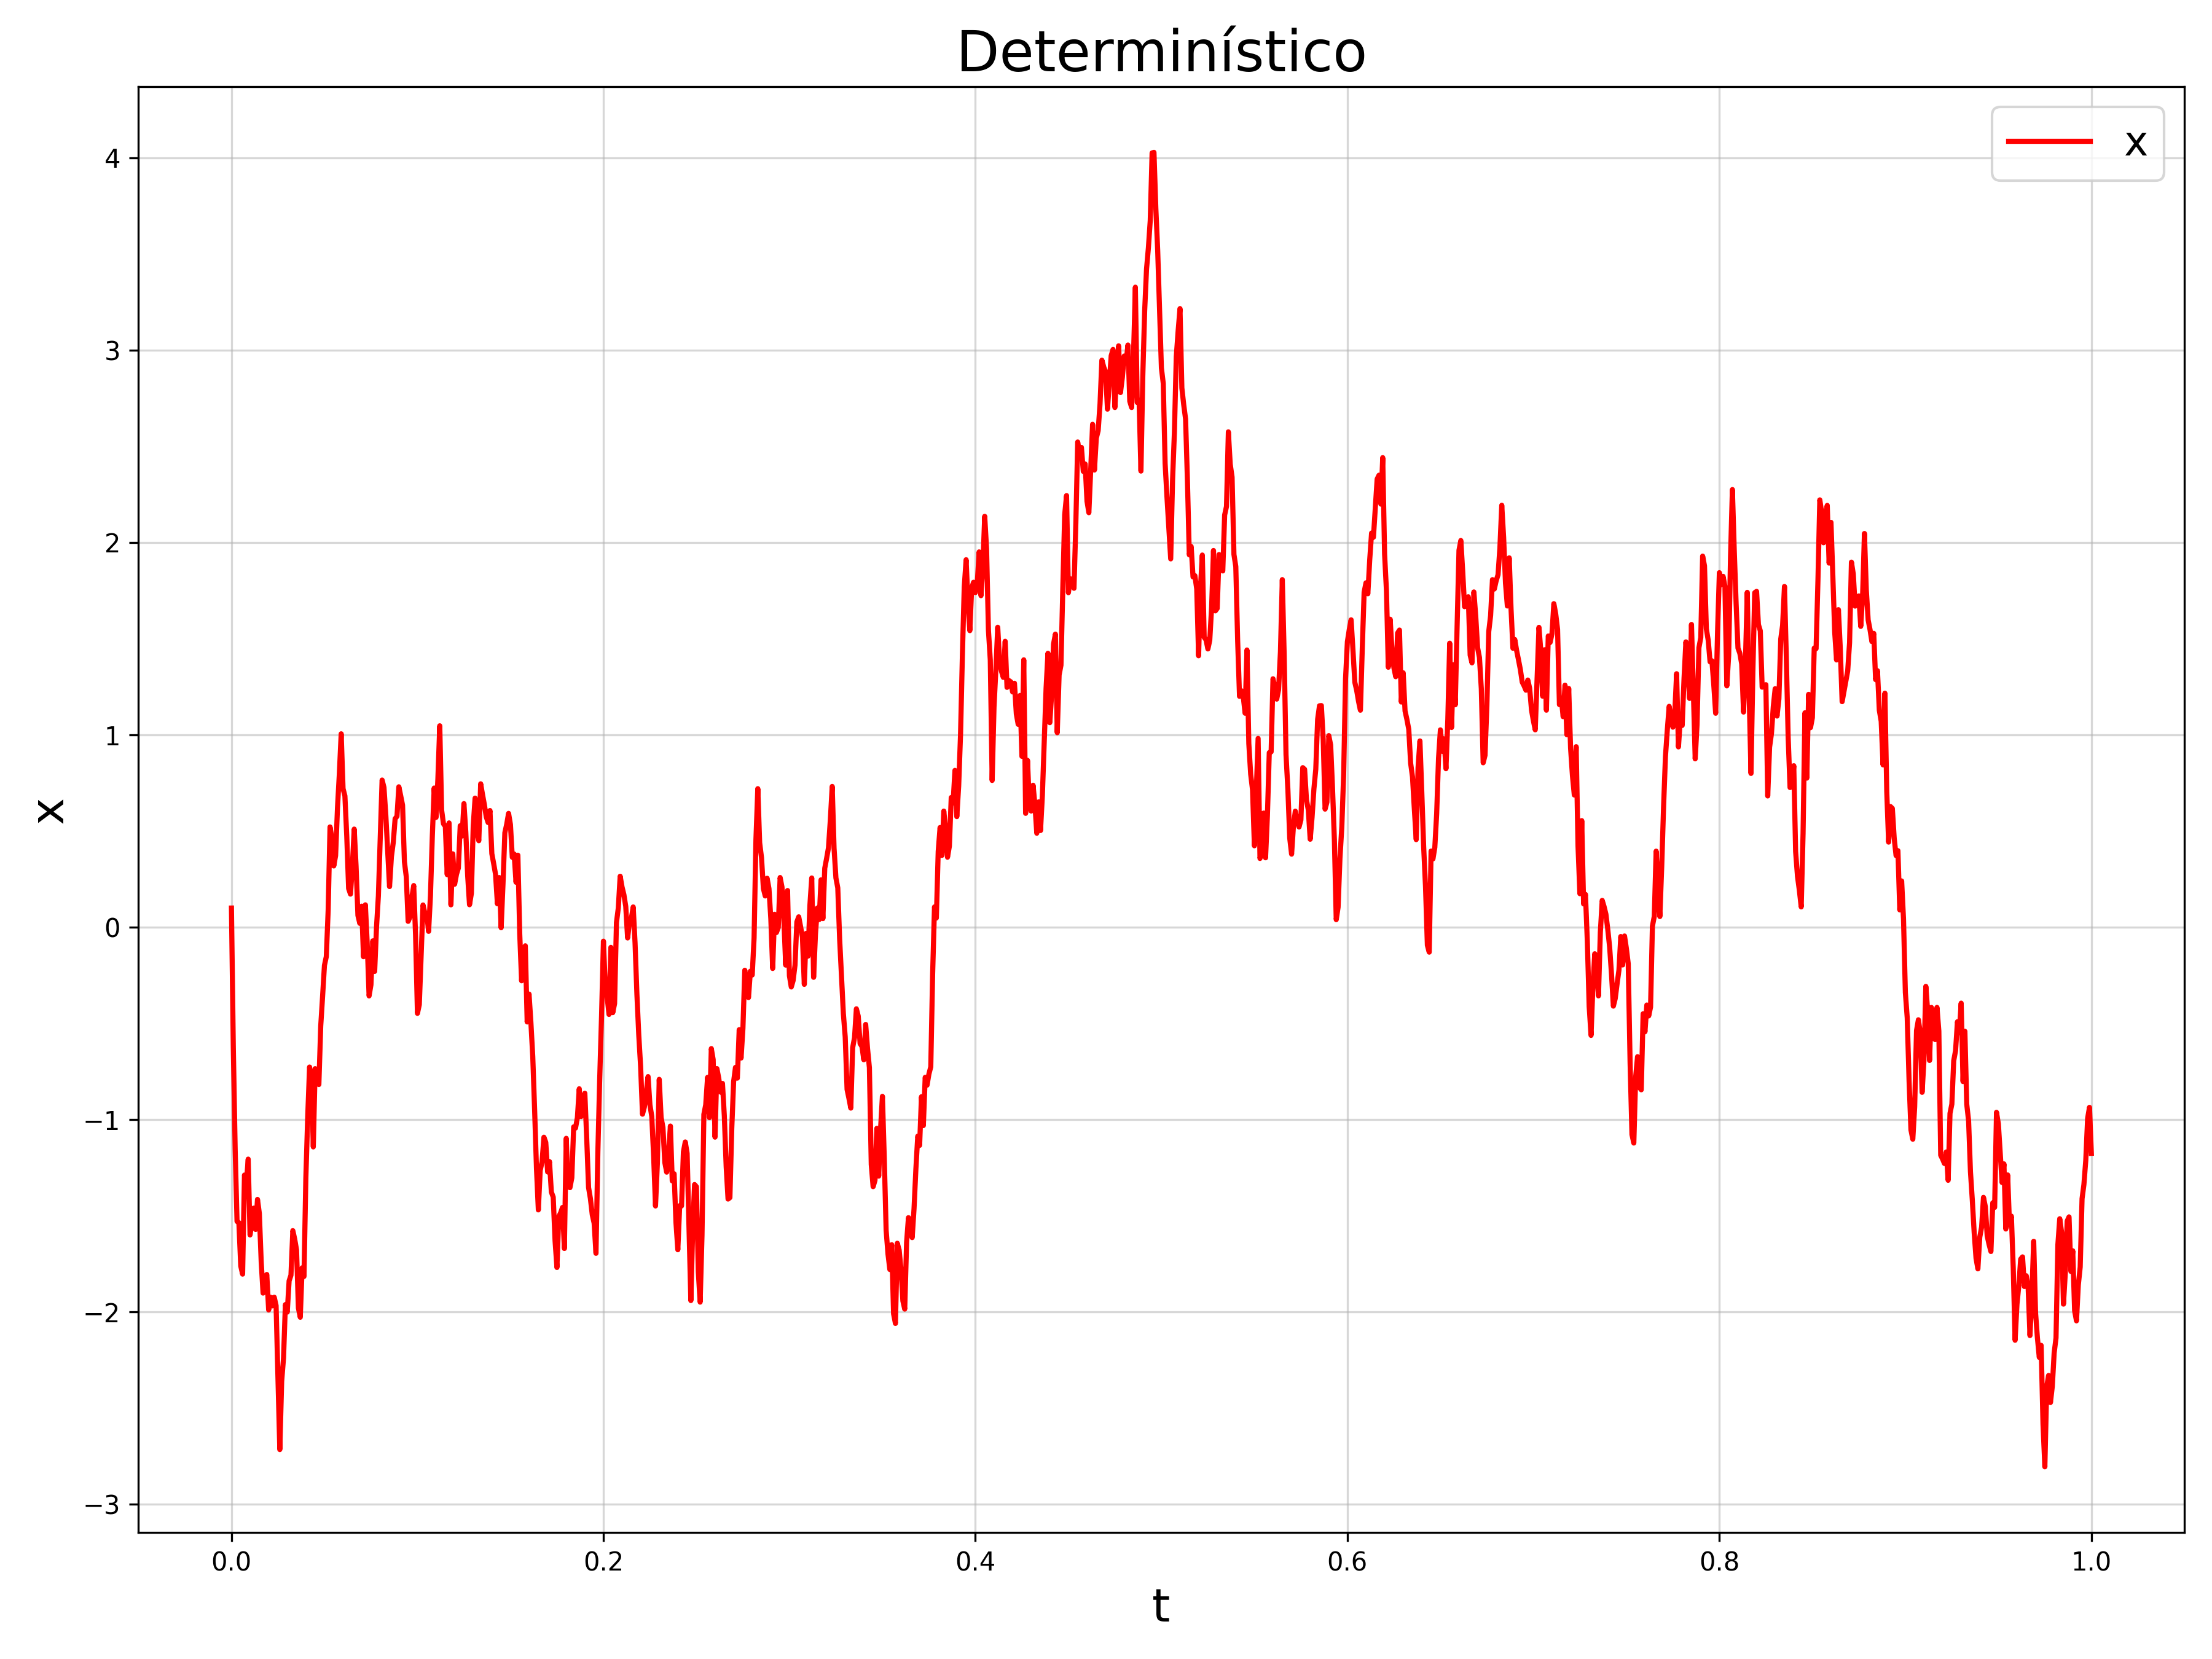
\includegraphics[width=0.45\textwidth]{00_TCC/01_LATEX/figuras/ch02_introducao_a_sde/deterministico_plot.png}
        \label{fig:ch02-exemplo-histograma-deterministico}
    }
    \hfill
    \subfloat[Browniano acoplado estocástico.]{
        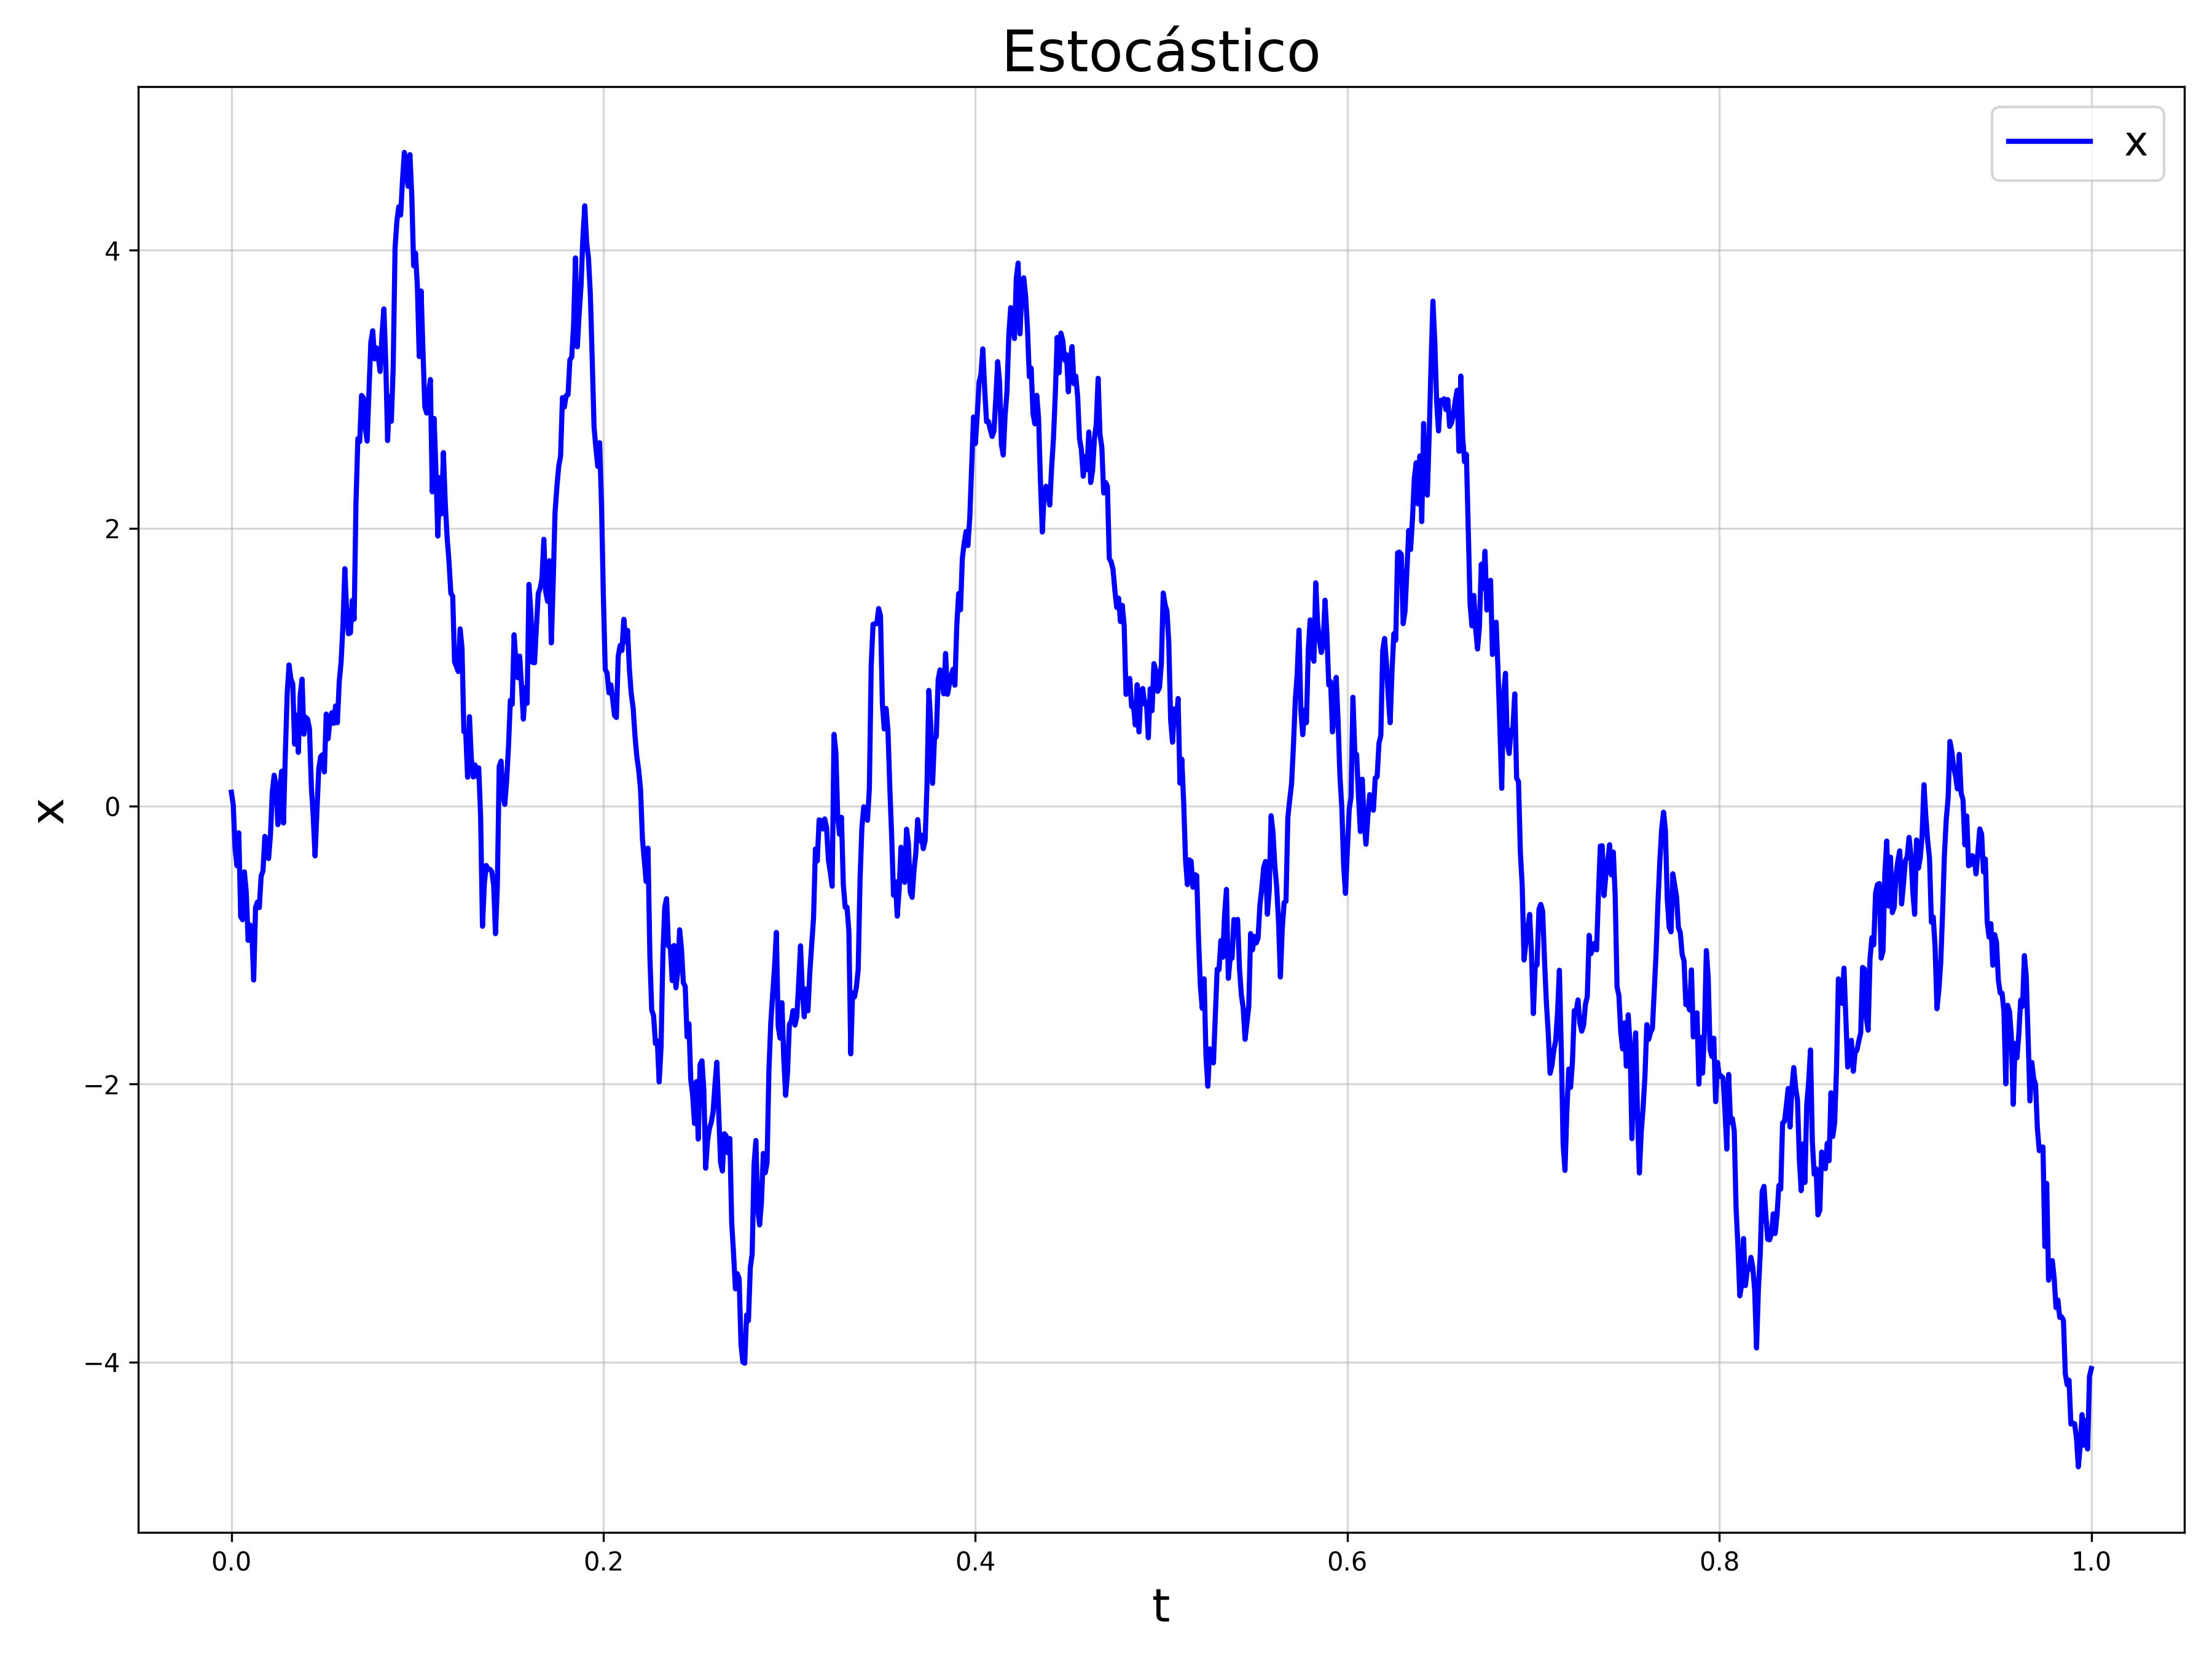
\includegraphics[width=0.45\textwidth]{00_TCC/01_LATEX/figuras/ch02_introducao_a_sde/estocastico_plot.png}
        \label{fig:ch02-exemplo-histograma-estocastico}
    }
    \caption{Comparação entre simulação determinística e estocástica do browniano acoplado.}
    \label{fig:ch02-exemplo-comparacao-simulacao}
\end{figure}

\begin{figure}[H]
    \centering
    \subfloat[Histograma do browniano acoplado determinístico.]{
        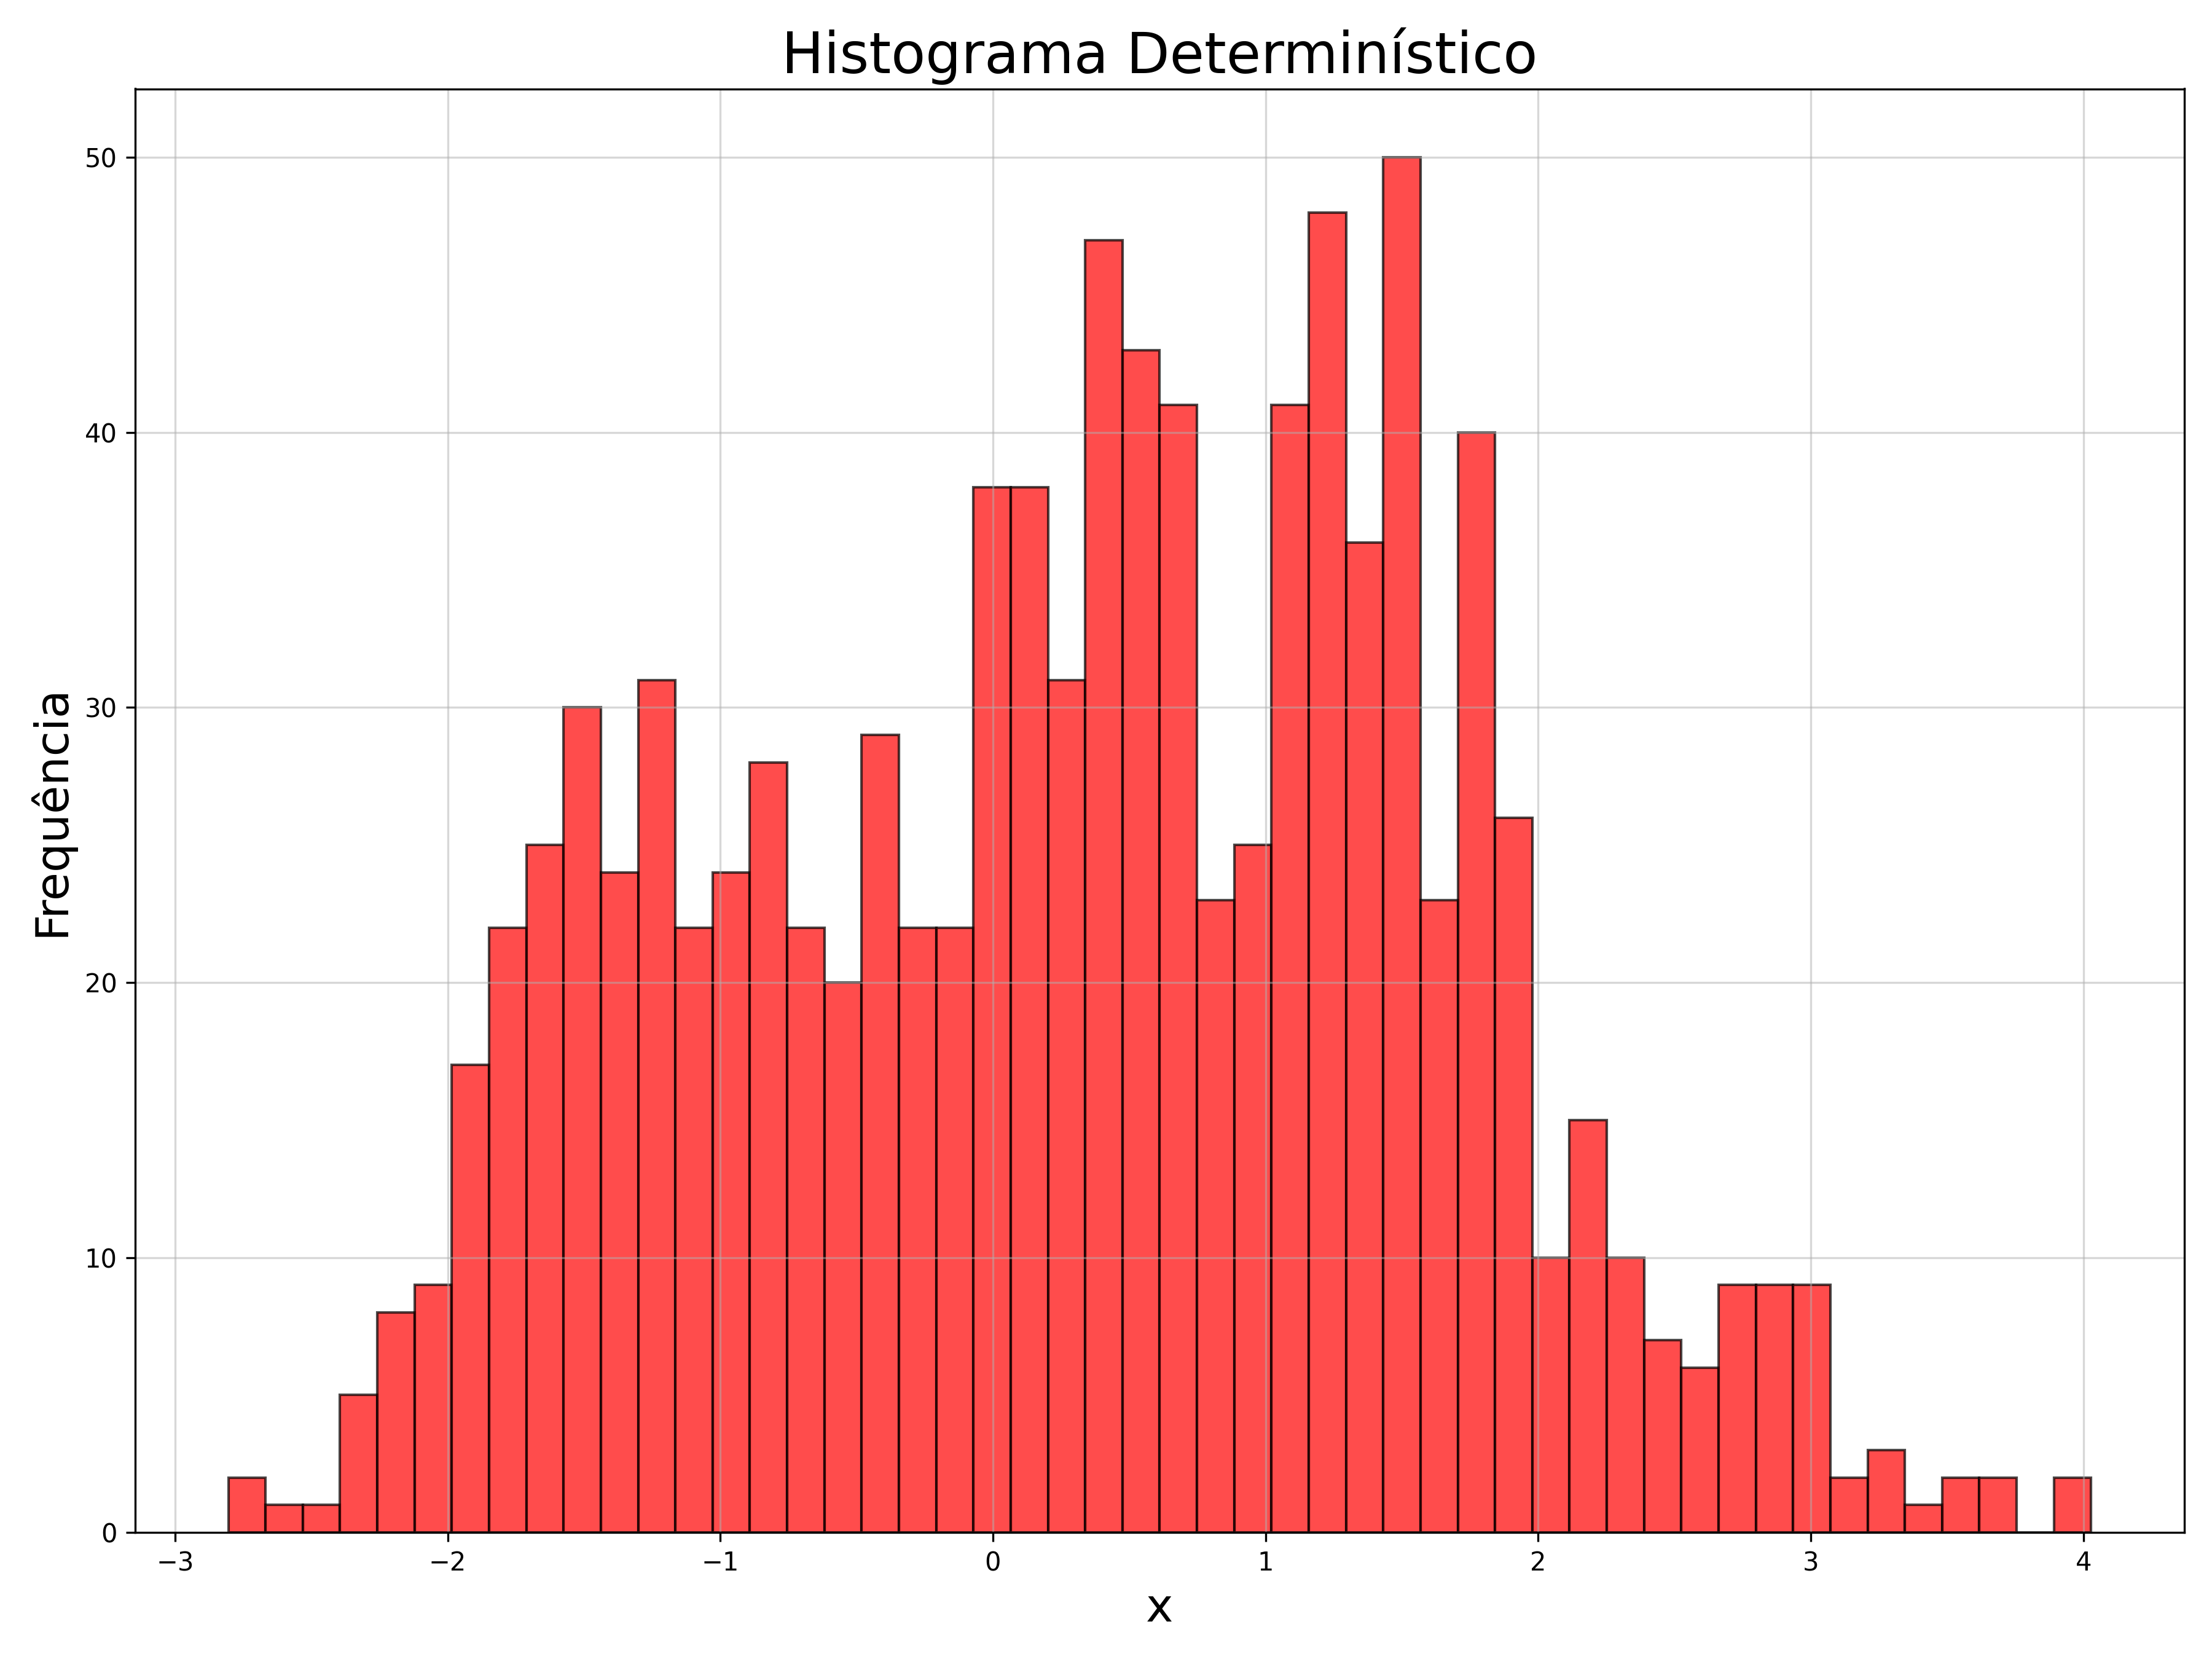
\includegraphics[width=0.45\textwidth]{00_TCC/01_LATEX/figuras/ch02_introducao_a_sde/hist_deterministico.png}
        \label{fig:ch02-exemplo-histograma-deterministico}
    }
    \hfill
    \subfloat[Histograma do browniano acoplado estocástico.]{
        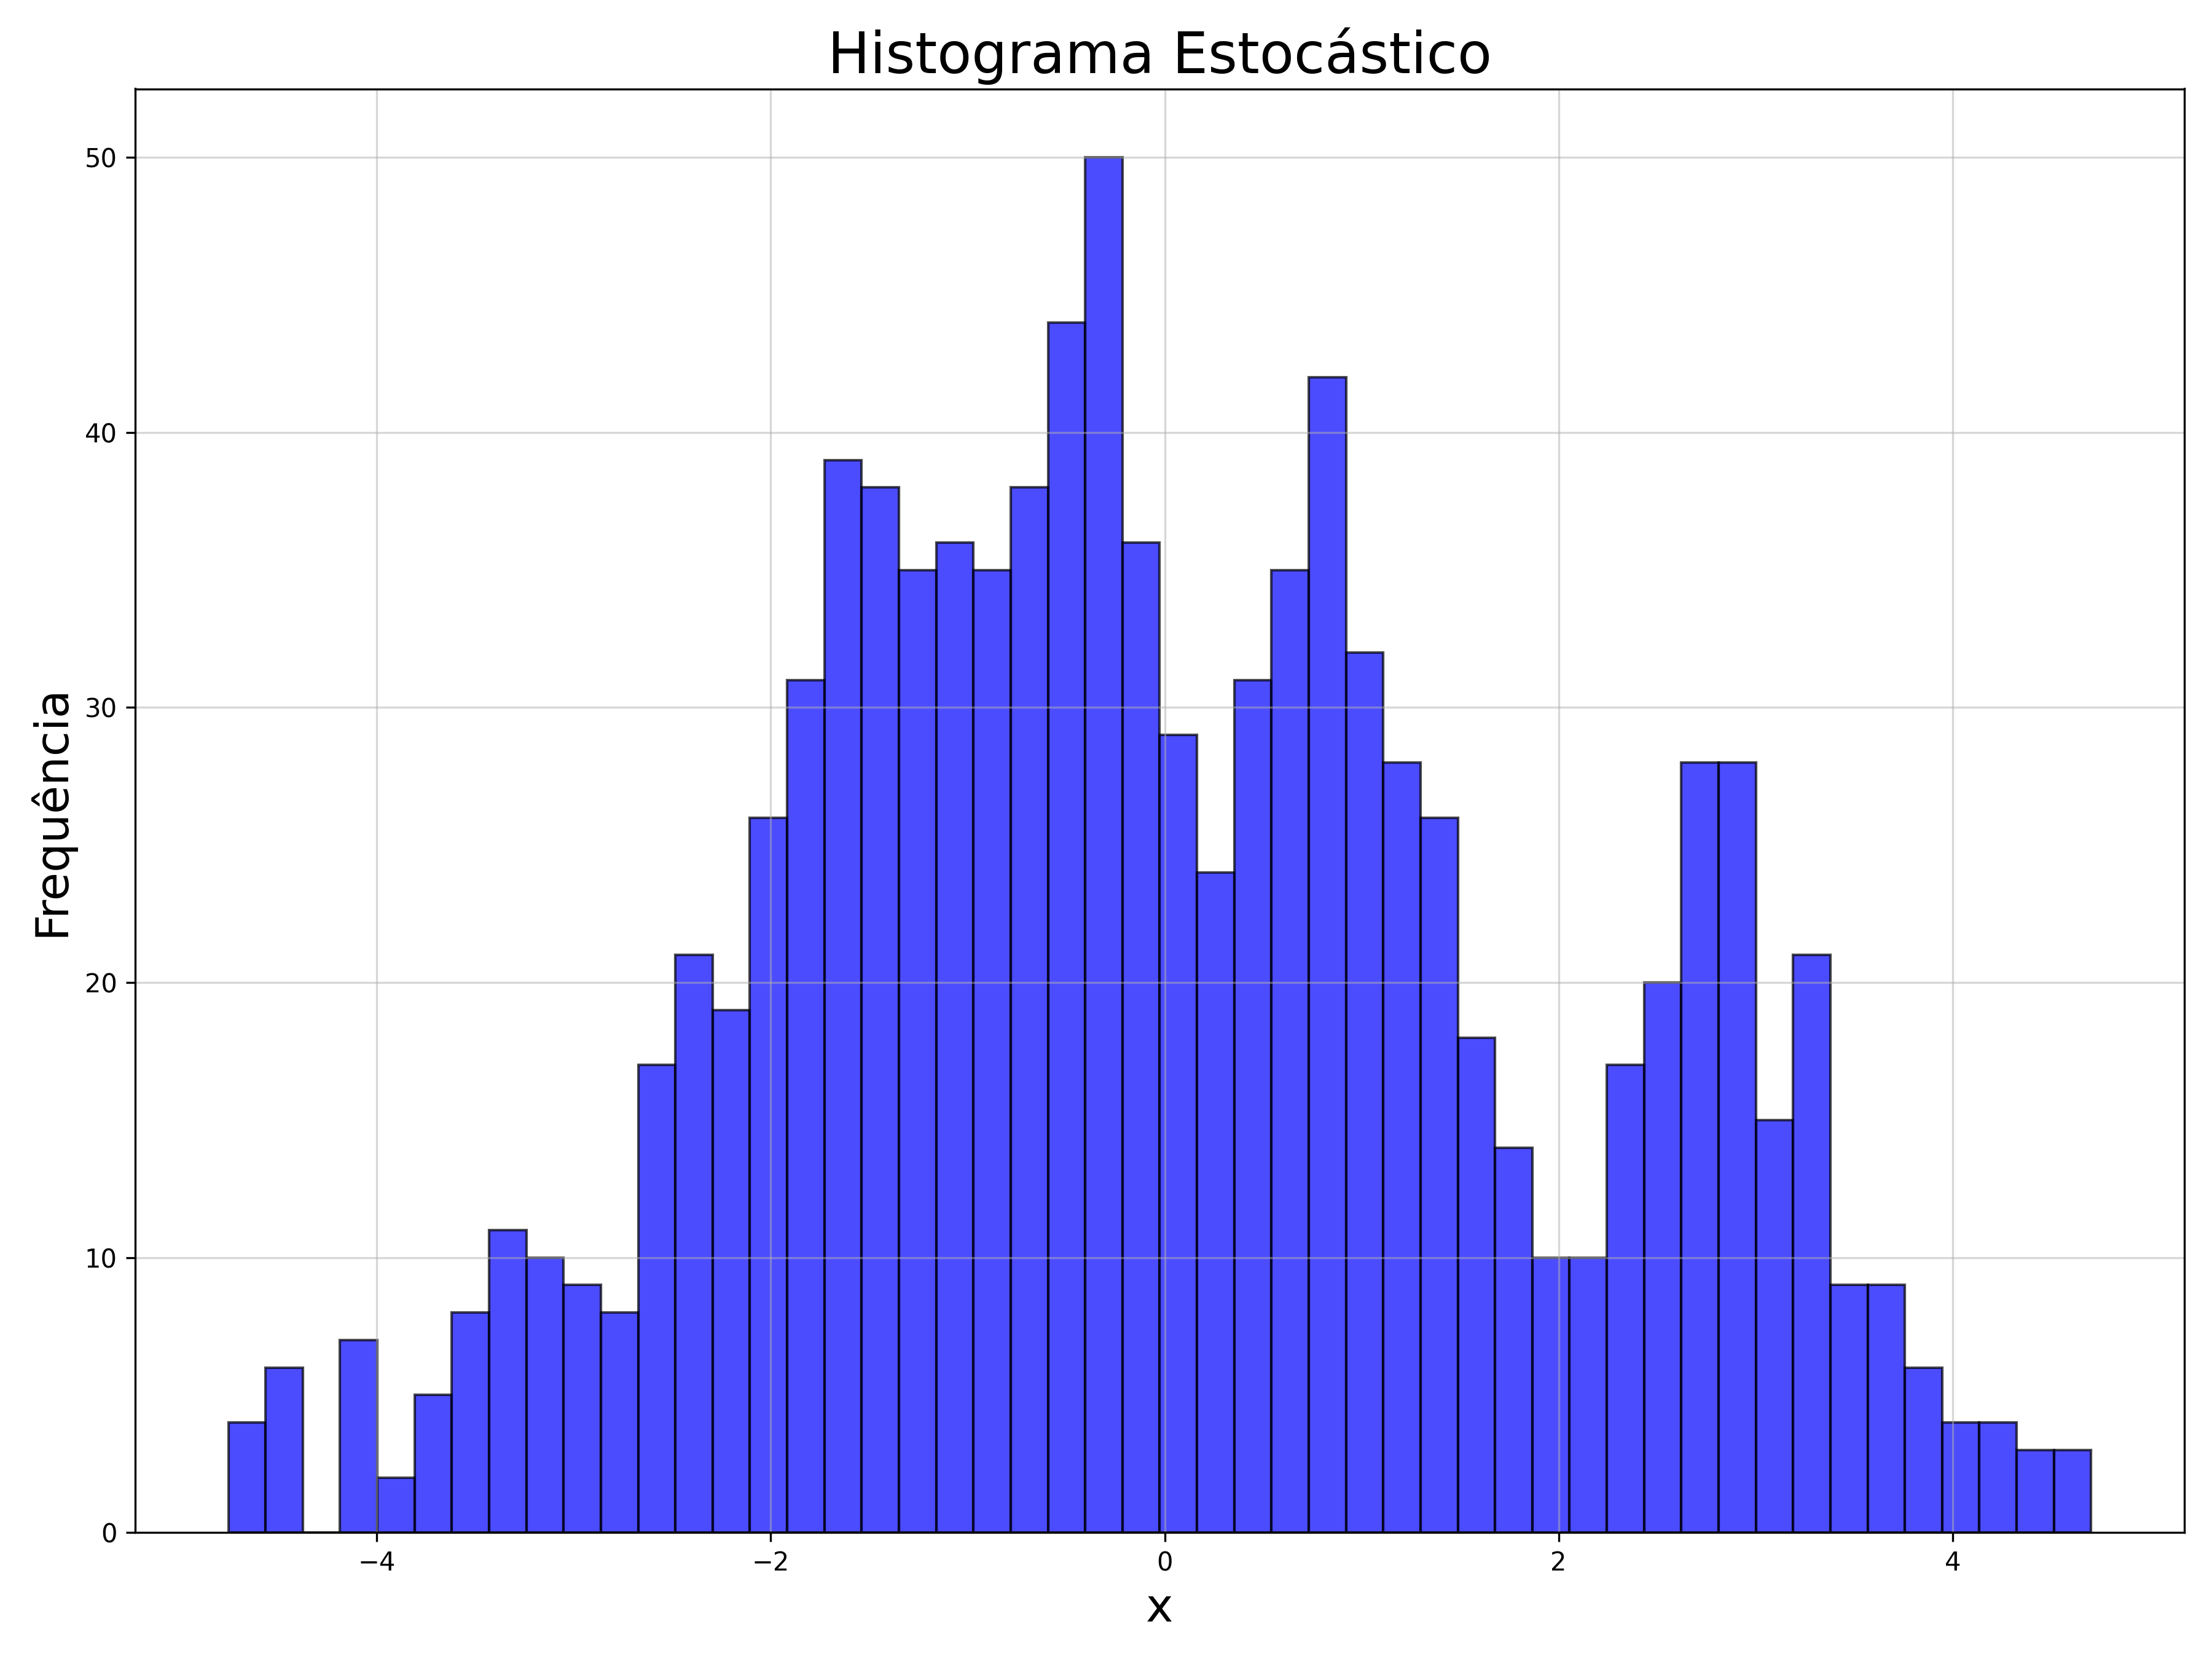
\includegraphics[width=0.45\textwidth]{00_TCC/01_LATEX/figuras/ch02_introducao_a_sde/hist_estocastico.png}
        \label{fig:ch02-exemplo-histograma-estocastico}
    }
    \caption{Comparação entre histogramas das simulações determinística e estocástica do browniano acoplado.}
    \label{fig:ch02-exemplo-comparacao-histogramas}
\end{figure}

